%% 
%% Copyright 2007, 2008, 2009 Elsevier Ltd
%% 
%% This file is part of the 'Elsarticle Bundle'.
%% ---------------------------------------------
%% 
%% It may be distributed under the conditions of the LaTeX Project Public
%% License, either version 1.2 of this license or (at your option) any
%% later version.  The latest version of this license is in
%%    http://www.latex-project.org/lppl.txt
%% and version 1.2 or later is part of all distributions of LaTeX
%% version 1999/12/01 or later.
%% 
%% The list of all files belonging to the 'Elsarticle Bundle' is
%% given in the file `manifest.txt'.
%% 

%% Template article for Elsevier's document class `elsarticle'
%% with numbered style bibliographic references
%% SP 2008/03/01

\documentclass[preprint,1p]{elsarticle}
\biboptions{numbers,sort&compress}

%% Use the option review to obtain double line spacing
%% \documentclass[authoryear,preprint,review,12pt]{elsarticle}

%% Use the options 1p,twocolumn; 3p; 3p,twocolumn; 5p; or 5p,twocolumn
%% for a journal layout:
%% \documentclass[final,1p,times]{elsarticle}
%% \documentclass[final,1p,times,twocolumn]{elsarticle}
%% \documentclass[final,3p,times]{elsarticle}
%% \documentclass[final,3p,times,twocolumn]{elsarticle}
%% \documentclass[final,5p,times]{elsarticle}
%% \documentclass[final,5p,times,twocolumn]{elsarticle}

%% For including figures, graphicx.sty has been loaded in
%% elsarticle.cls. If you prefer to use the old commands
%% please give \usepackage{epsfig}

%% The amssymb package provides various useful mathematical symbols
\usepackage{amssymb}
\usepackage{lineno}
\usepackage{hyperref}
%% The amsthm package provides extended theorem environments
%% \usepackage{amsthm}

%% The lineno packages adds line numbers. Start line numbering with
%% \begin{linenumbers}, end it with \end{linenumbers}. Or switch it on
%% for the whole article with \linenumbers.
%% \usepackage{lineno}

\journal{Nucl. Instrum. Meth. A}

\begin{document}
\linenumbers

\begin{frontmatter}

%% Title, authors and addresses

%% use the tnoteref command within \title for footnotes;
%% use the tnotetext command for theassociated footnote;
%% use the fnref command within \author or \address for footnotes;
%% use the fntext command for theassociated footnote;
%% use the corref command within \author for corresponding author footnotes;
%% use the cortext command for theassociated footnote;
%% use the ead command for the email address,
%% and the form \ead[url] for the home page:
%% \title{Title\tnoteref{label1}}
%% \tnotetext[label1]{}
%% \author{Name\corref{cor1}\fnref{label2}}
%% \ead{email address}
%% \ead[url]{home page}
%% \fntext[label2]{}
%% \cortext[cor1]{}
%% \address{Address\fnref{label3}}
%% \fntext[label3]{}

\title{Cadmium Telluride Sensor}

%% use optional labels to link authors explicitly to addresses:
%% \author[label1,label2]{}
%% \address[label1]{}
%% \address[label2]{}

\author[2]{A.~Apresyan}
\author[1]{A.~Bornheim}
\author[1]{C.~Pena}
\author[1]{M.~Spiropulu}
\author[1]{S.~Xie}
\author[1]{Z.~Zhang}
\address[1]{California Institute of Technology, Pasadena, CA, USA}
\address[2]{Fermi National Accelerator Laboratory, Batavia, IL, USA}
\cortext[cor]{Corresponding author}

\begin{abstract}
%% Text of abstract


\end{abstract}

\begin{keyword}
%% keywords here, in the form: keyword \sep keyword

%% PACS codes here, in the form: \PACS code \sep code
Silicon \sep Timing \sep Calorimeter
%% MSC codes here, in the form: \MSC code \sep code
%% or \MSC[2008] code \sep code (2000 is the default)

\end{keyword}

\end{frontmatter}

%% \linenumbers

%% main text
\section{Introduction} 

 
\section{Cadmium Telluride Sensor}
\label{sec:siliconpad}

%Fig: Quantum Efficiency vs wavelength
%Photos of sensor, drawing for the circuit

  
\section{Test-beam Setup and Experimental Apparatus }
\label{sec:tbeam}

We performed the test-beam measurements at the H2 beamline of the CERN North-Area testbeam facility
and the T9 beamline of the CERN East-Area testbeam facility. They provide secondary electron beams 
from the Proton Synchrotron (PS) and Super Proton Synchrotron (SPS)
of energies ranging from $2$~GeV to $200$~GeV. The secondary beams are composed of 
a mixture of electrons, pions, and muons. 

Trigger counters made of photomultipliers coupled to plastic scintillators are used 
to initiate the read out of the data acquisition (DAQ) system. The DAQ system
uses a CAEN V1742 switched capactor digitizer based on the DRS4 chip. Gas wire chambers
are used to measure the position of each incident beam particle in the plane transverse
to the beamline. A stack of lead or tungsten absorbers of different thicknesses are 
placed about $5$~mm in front of the Cadmium Telluride (CdTe) sensor, which is 
enclosed within a metal box covered by copper foil. A micro-channel plate photomultiplier (MCP-PMT)
detector is used to provide a very precise reference timestamp. At the T9 beamline,
a Hamamatsu R3809U MCP-PMT is placed just upstream of the absorber material. 
At the H2 beamline a Photek 240 MCP-PMT is used, which contains a significant 
amount of absorber material (about 1.8 radiation lengths), and is therefore placed 
just downstream of the CdTe sensor to avoid inducing an early electromagnetic shower.
The precision of the time measurement for both types of MCP-PMT's is less than 
$10$~ps~\cite{Ronzhin2015288}. The purity of the electron beam at the T9 beamline is
significantly lower than at the H2 beamline, and therefore we use a LYSO crystal
optically coupled to an MCP-PMT as a means of discriminating the electrons from the pions
in the beam. The schematic diagrams of the experimental setups at H2 and T9 
are shown in Figure~\ref{fig:BeamSchematicDiagram}. 


%Fig: Diagram of detector elements
\begin{figure}[htbp] 
\centering
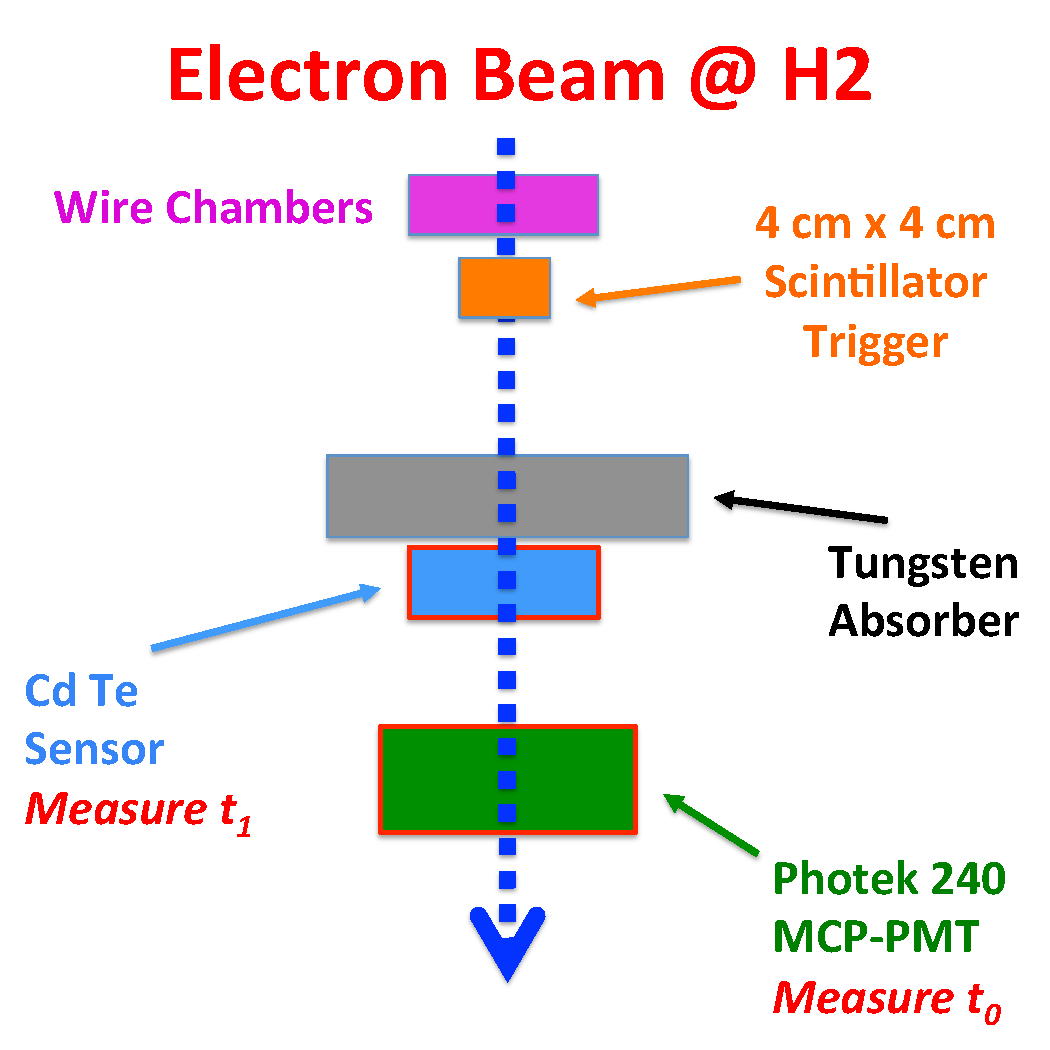
\includegraphics[width=0.49\textwidth]{figures/H2_BeamSchematicDiagram.pdf} 
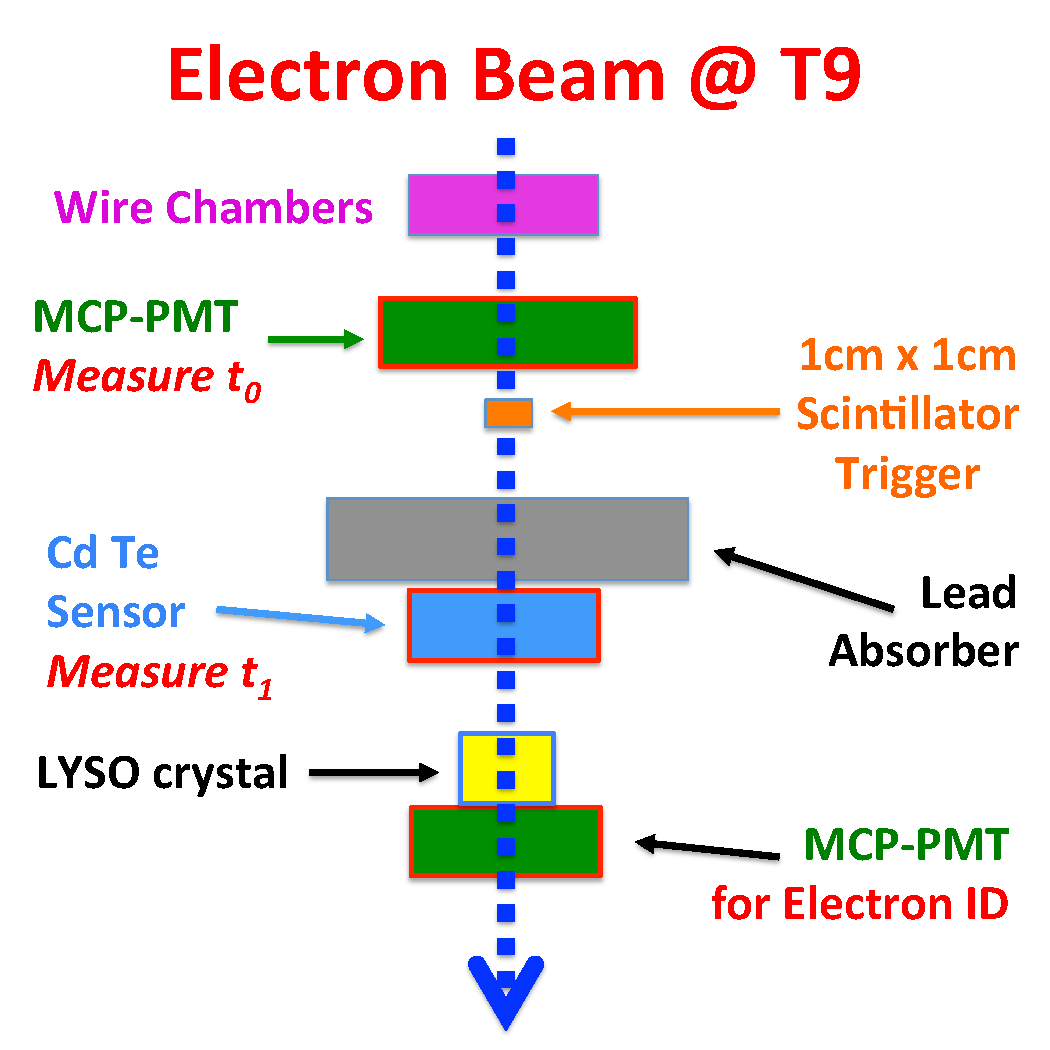
\includegraphics[width=0.49\textwidth]{figures/T9_BeamSchematicDiagram.pdf} 
\caption{Schematic diagrams of the test-beam setups at H2 (left) and T9 (right) are shown. 
The timestamps $t_0$ and $t_1$ are defined in Section~\ref{sec:results}.} 
\label{fig:BeamSchematicDiagram} 
\end{figure} 


The X and Y position measurements from the wire chamber are used to determine the location
of the CdTe sensor relative to the beam and to align the beam. In 
Figure~\ref{fig:BeamSensorPosition}, we show plots of the average amplitude measured in the
CdTe sensor as a function of the X and Y positions as measured by the wire chamber. Based
on these plots, we can restrict our measurements to the electrons whose impact point is close
to the center of the CdTe sensor.

%Fig: Beam profile X-Y plot
\begin{figure}[htbp] 
\centering
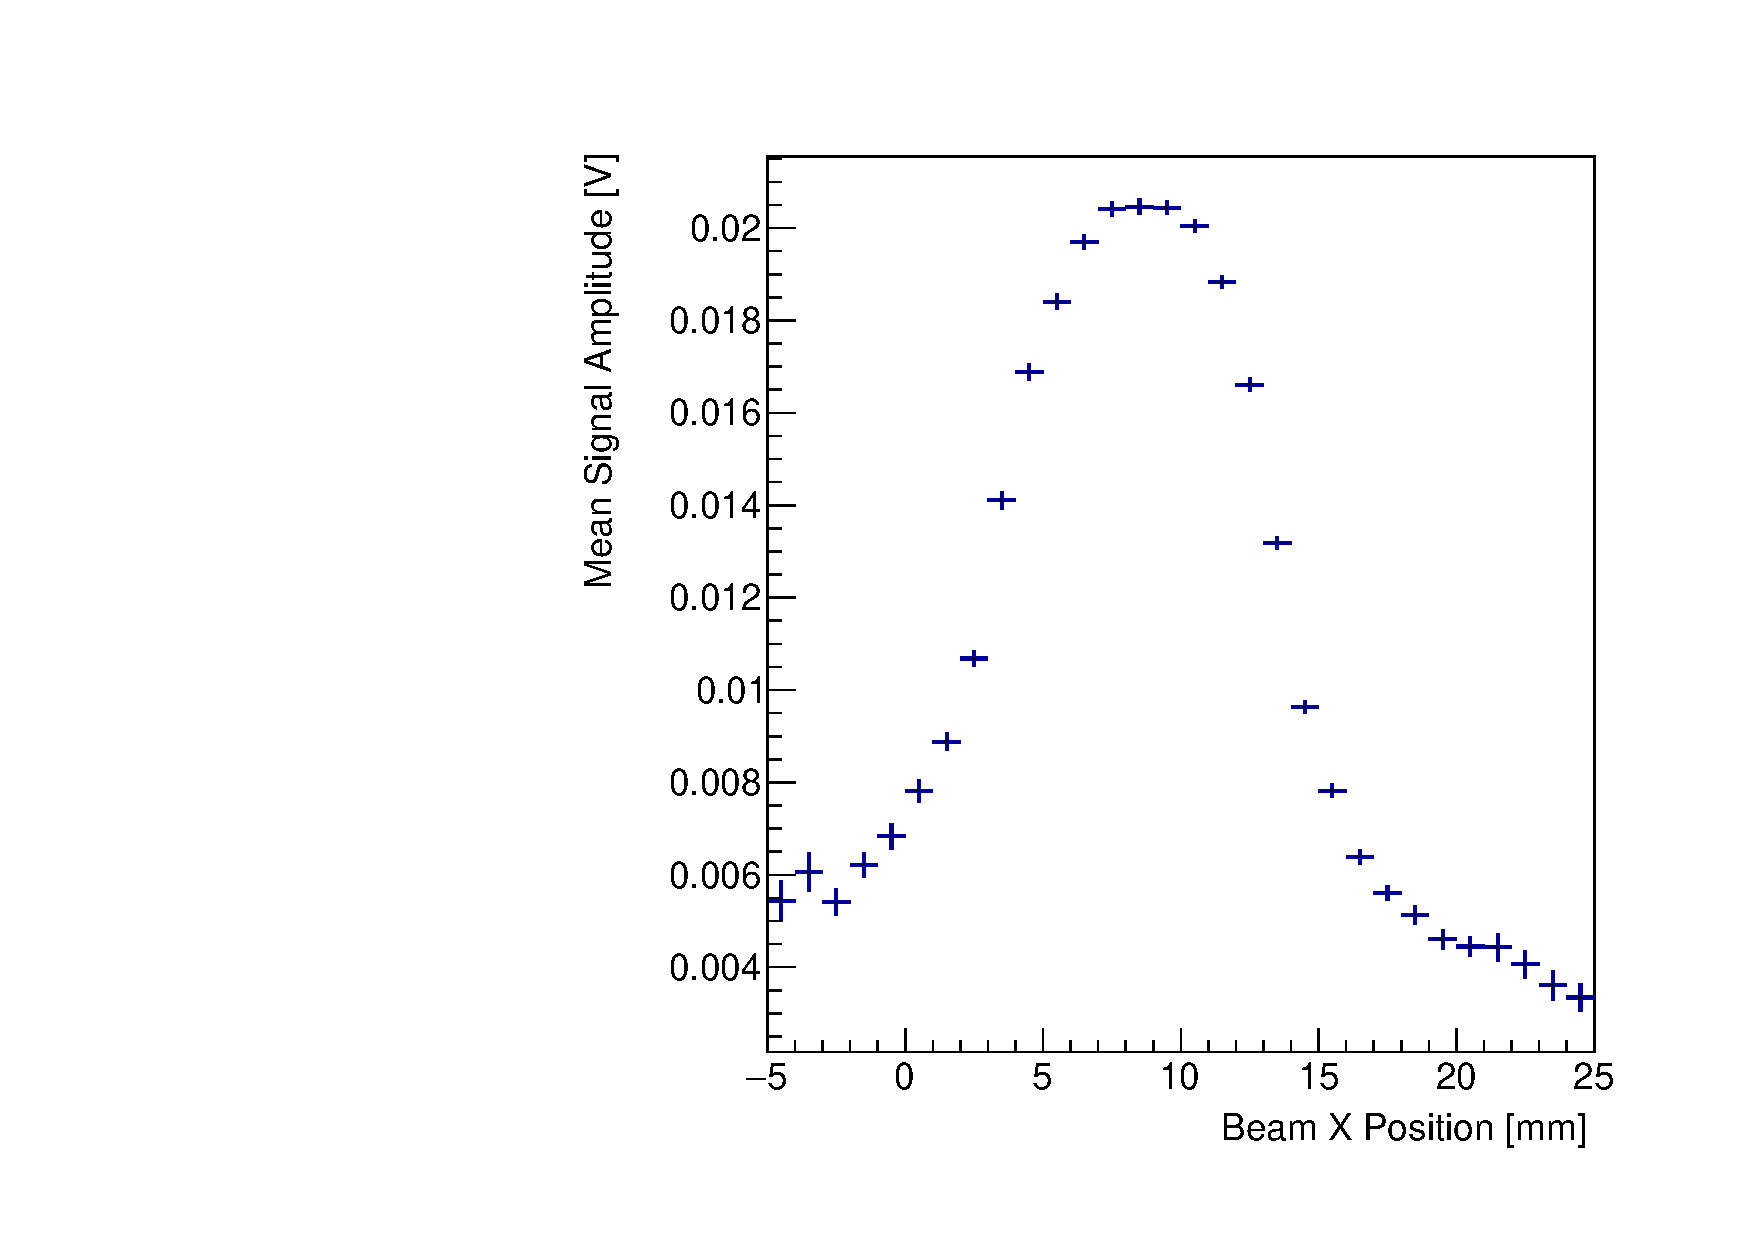
\includegraphics[width=0.49\textwidth]{figures/SensorXProfile.pdf} 
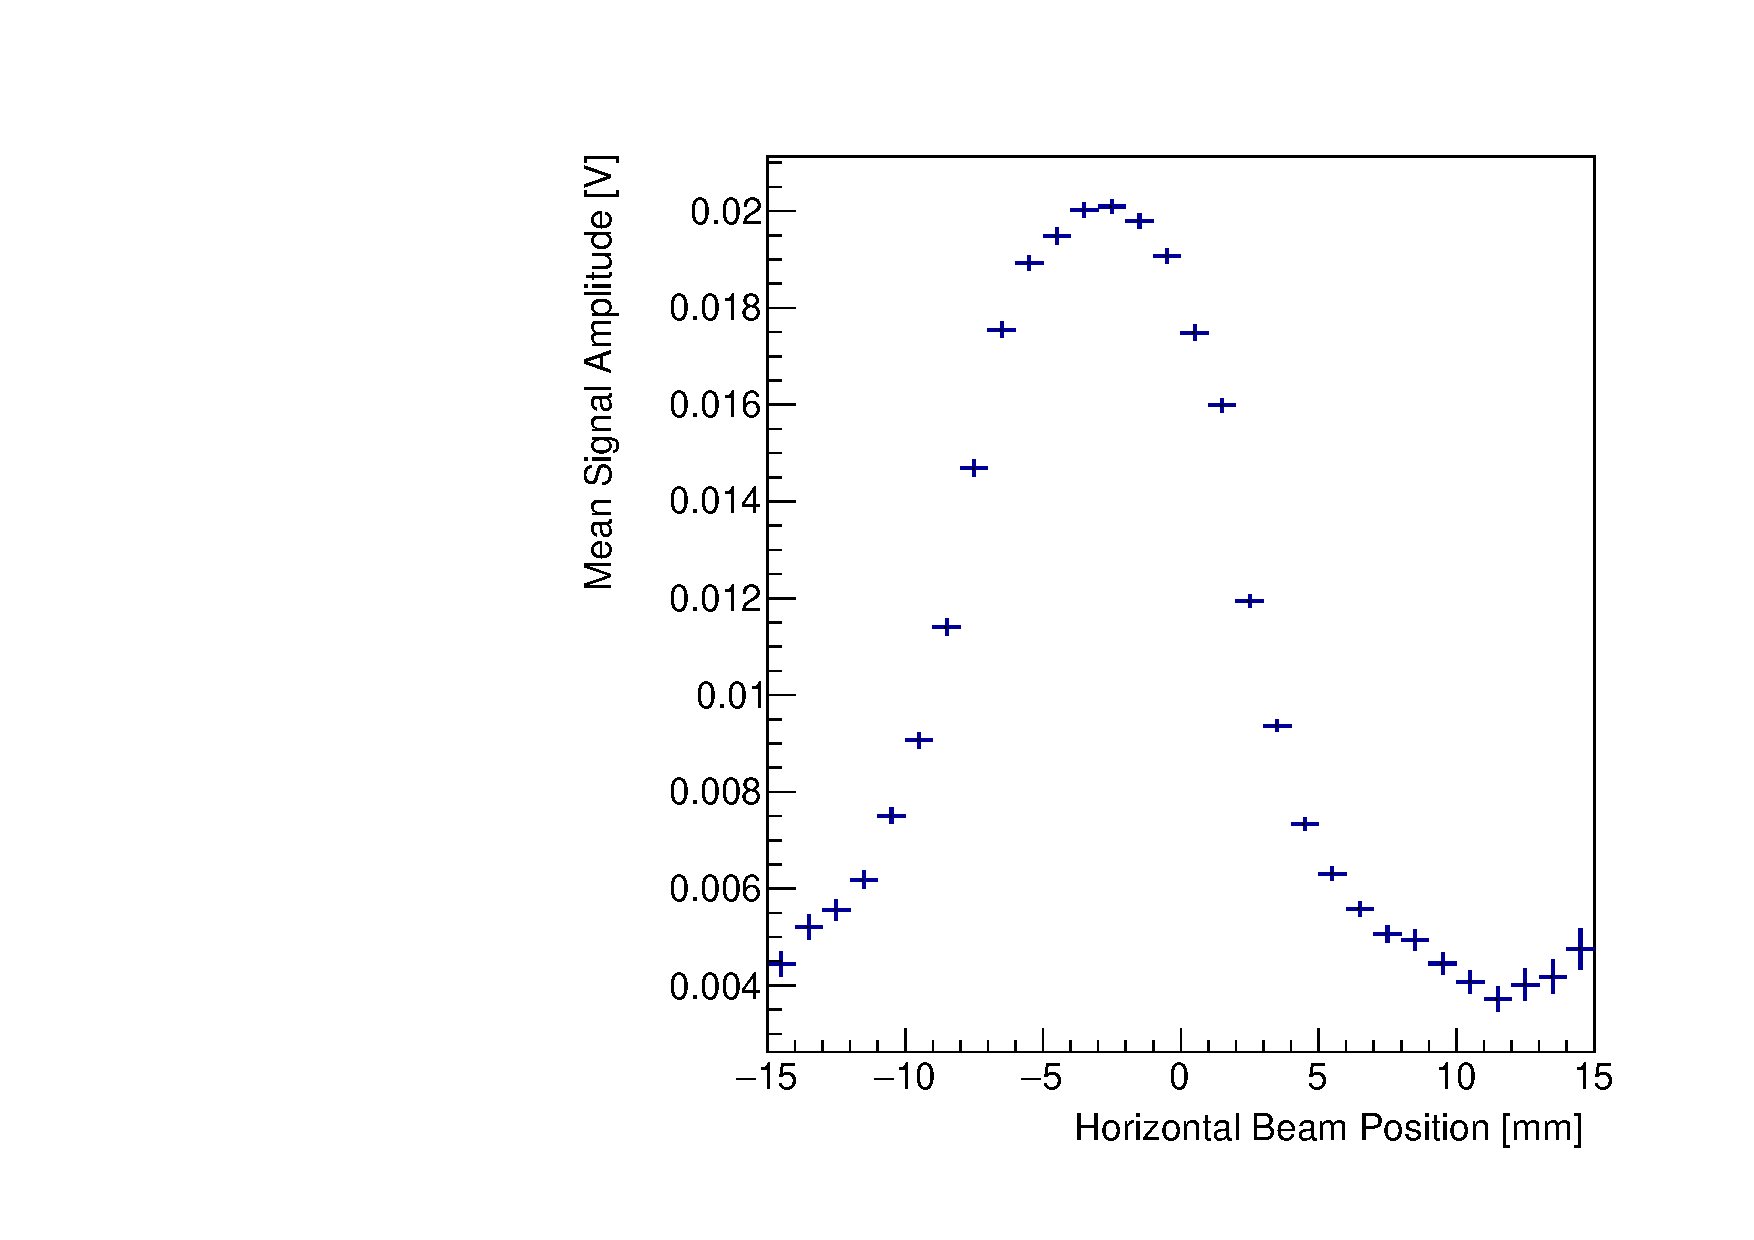
\includegraphics[width=0.49\textwidth]{figures/SensorYProfile.pdf} 
\caption{The average amplitude measured in the CdTe sensor is plotted as a function of 
the X and Y positions of the beam particle as measured by the wire chamber.} 
\label{fig:BeamSensorPosition} 
\end{figure} 



\section{Test Beam Measurements and Results} 
\label{sec:results} 


%Fig: Pulse shapes for various energies
\begin{figure}[htbp] 
\centering
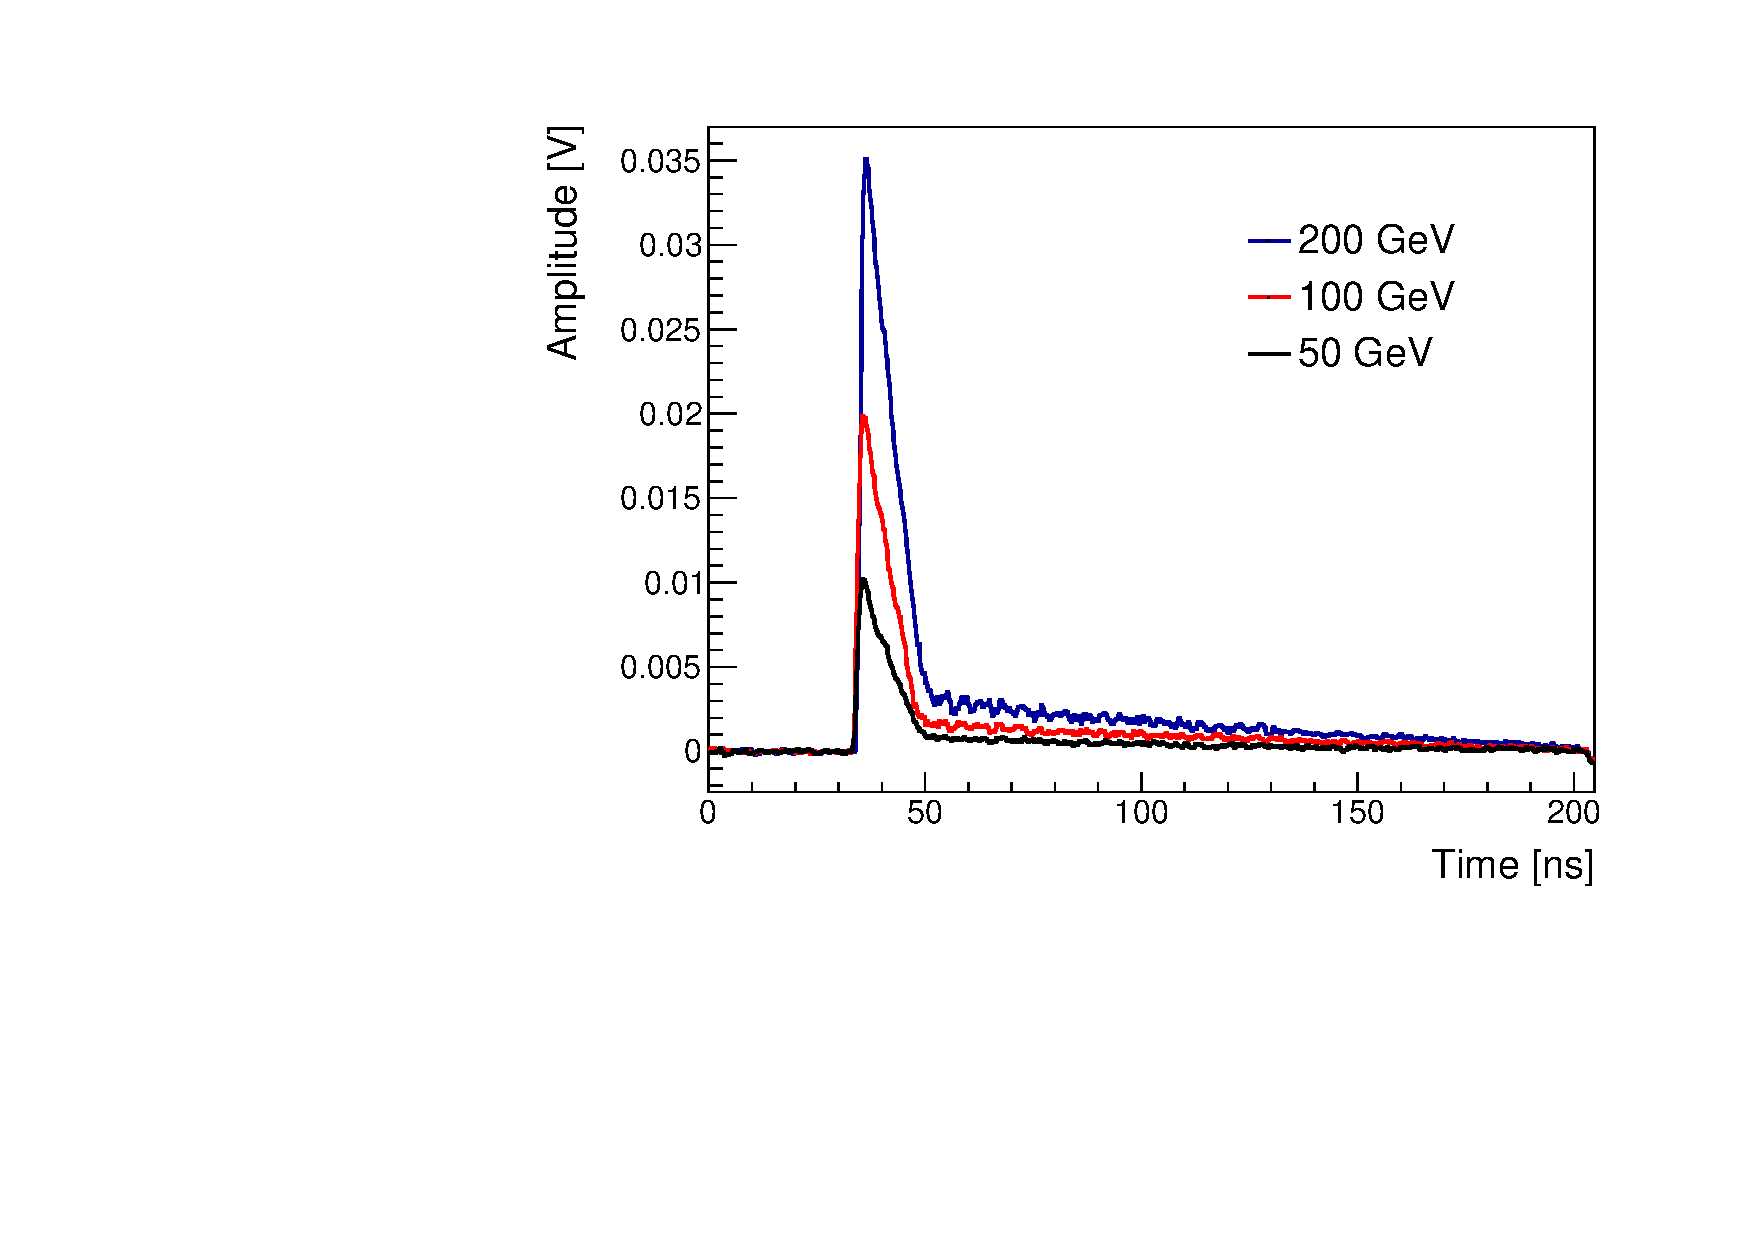
\includegraphics[width=0.75\textwidth]{figures/TypicalPulses.pdf} 
\caption{Examples of signal pulses in the CdTe sensor for electrons with energies of $50$~GeV,
$100$~GeV, and $200$~GeV.} 
\label{fig:Pulses} 
\end{figure} 




%Fig: Charge distributions (noise, showers, MIP?)
%Fig: Collected Charge vs Beam Energy

%Fig: example DeltaT plot
%Fig: Time resolution vs beam energy

%Extra studies
%Rise time vs beam energy
%DeltaT vs beam location
%DeltaT vs amplitude
%Charge vs beam location ( can we say anything about signal size on shower periphery? )

\section{Discussion} 
\label{sec:discussion} 


\section{Conclusion}
\label{sec:conclusion} 


%% The Appendices part is started with the command \appendix;
%% appendix sections are then done as normal sections
%% \appendix

%% \section{}
%% \label{}

%% If you have bibdatabase file and want bibtex to generate the
%% bibitems, please use
%%
%%  \bibliographystyle{elsarticle-num} 
%%  \bibliography{<your bibdatabase>}

%% else use the following coding to input the bibitems directly in the
%% TeX file.

\bibliography{CdTeCalorimeter}{}
\bibliographystyle{ieeetr} 

%\begin{thebibliography}{00}

%% \bibitem{label}
%% Text of bibliographic item

%\bibitem{}

%\end{thebibliography}

\end{document}
